
\documentclass[main.tex]{subfiles}

\begin{document}

\chapter{Onset of inelasticity in a continuum}
\label{LEC:ContinuumInelasticity}

\section{Representation of strain and strain in a continuum}
\label{Sec:tensor_representation}
To achieve strain softening and localization in standard finite element analysis with continuous approximation of stress and strain fields we need to define a failure criterion as a scalar equation in a material point. In 1D models of the bond behavior, the onset of inelasticity has been 
defined in terms of slip $s$ and shear stress $\tau$. Similarly, the 1D models of crack localization used  strain $\epsilon$ and stress $\sigma$ in the direction of tensile loading. However, in a 2D an 3D continuum the stress and strain state of a material point is characterized by non-scalar variables, i.e. strain tensor 
$\boldsymbol{\varepsilon} = \varepsilon_{ij}$ and stress tensor $\boldsymbol{\sigma} = \sigma_{ij}$.
Tensors represent the state of a material frame within a continuum using six and nine variable components 
in 2D and 3D continuum, respectively.

Consider a strain tensor in 3D
\begin{align}
    \label{3d_strain_tensor}
    \boldsymbol{\varepsilon} = \varepsilon_{ij} =
    \left[    
    \begin{array}{ccc}
         \varepsilon_{11} & \varepsilon_{12} & \varepsilon_{13}  \\
         \varepsilon_{21} & \varepsilon_{22} & \varepsilon_{23}  \\
         \varepsilon_{31} & \varepsilon_{32} & \varepsilon_{33}  \\
    \end{array}
    \right]
\end{align}
To introduce a failure criteria in 2D and 3D as a scalar equation of the form 
$f(\boldsymbol{\varepsilon})=0$ or $f(\boldsymbol{\sigma})=0$ we need to define measures 
of strain and stress tensor. Thus, we need to combine the information stored in a tensor
to obtain a single number deciding whether or not the material state is elastic or inelastic.
This task requires some understanding of the way a tensor stores the information about the
material deformation.

To do that, we exploit two properties of a tensor:
\begin{itemize}
\item
The strain tensor is symmetric, thus $\varepsilon_{ij} = \varepsilon_{ji}$. As a result, 
there are only six independent variables included in the strain tensor given in expression \ref{3d_strain_tensor}). 
\item
The tensor in expression (\ref{3d_strain_tensor}) describes the deformation of a material
state from a particular position of an observer. In other words, the
tensor representation is related to a particular coordinate system. If the observer 
changes the position, he or she will see the deformed cube with different values
of the components. However, the deformation of the material frame did not change.
Thus, there must some values hidden in the tensor representation that are invariant
with respect to the coordinate system.
\end{itemize}

\mnote{Basic invariants}
Indeed, strain tensor describes the volume and shape change of a unit material frame and this
change can be captured using three invariants of a tensor.
Volumetric strain is obtained as an average of the normal strain components, i.e.
\begin{align}
\label{EQ:first_strain_invariant}
    I_1 =  \varepsilon_{xx} + \varepsilon_{yy} + \varepsilon_{zz}
\end{align}
It is convenient to write this expression in an indicial notation using the so called Einstein summation rule,  making the mathematical expressions directly "programmable". We shall use the index notation to directly visualize the yield surfaces and study the differences between them.
The first strain invariant given in (\ref{EQ:first_strain_invariant}) can be rewritten in index notation as
\begin{align}
\label{eq:I_1}
    I_1 = \varepsilon_{ii}
\end{align}
The Einstein summation rule introduces an implicit summation over the terms with repeated indexes. 
The above expression is then evaluated as
\[
  I_1 = \sum_{i=1}^{3} \sigma_{ii}
\]
There are another two invariants $I_2$, $I_3$ that capture the change of shape of a material frame.
Their definition is given as
\begin{align}
\label{eq:I_2}
I_2 &= \frac{1}{2} \left[ \varepsilon_{kk}^2 - \varepsilon_{ij}\varepsilon_{ij} \right] \\
\label{eq:I_3}
I_3 &= \epsilon_{ijk} E_{i1} E_{j2} E_{k3}.
\end{align}

\mnote{Demo script}
Using \lstin{numpy} package we can apply directly this convention also in coding a mathematical expression. The first invariant of the stress tensor is then expressed as
\begin{lstlisting}[name=Calsulation of the first strain tensor invariant, frame=none]
import numpy as np
epsilon = np.array([[1.0, 2.1, 3.5],
                  [2.1, 3.0, 1.2],
                  [3.5, 1.2, 2.0], dtype=np.float_)
I_1 = np.einsum('ii', epsilon)
print 'I_1', I_1
\end{lstlisting}
For some examples of strain tensor invariants and their behavior and evaluation see
the interactive page\\
\href{http://www.continuummechanics.org/principalstrain.html}{http://www.continuummechanics.org/principalstrain.html}.  

\mnote{Changing the position of observer}
When we change the position of the observer, the invariants must not change. 
This means that the transformation rules of a tensor must keep the invariants untouched.
Such transformation matrix is achieved using the directional cosines representing the 
rotation between two Cartesian coordinate systems $x^{\prime}_i$ and $x_i$ 
\begin{align}
Q_{ij} = \cos(x_i^{\prime}-x_j).
\end{align}
Using such a transformation matrix, a tensor can be transformed using the rule
\begin{align}
\label{eq_tensor_transform}
\varepsilon^{\prime}_kl &= Q_{ki} Q_{li} \varepsilon_{ij}.
\end{align}
For details and exercises on tensor invariants and tensor transformation 
use standard literature on continuum mechanics. An interactive page 
with the explanation of the strain tensor transformations is provided at
the interactive page\\
\href{http://www.continuummechanics.org/coordxforms.html}{http://www.continuummechanics.org/coordxforms.html}

\mnote{Principal strains}
There is one special position of an observer that is very useful
for the introduction of failure criteria and for their visualization, namely the
perspective, in which the off-diagonal components of the tensor, i.e. 
$\varepsilon_{ij}, i\neq j$ vanish. 
In this configuration, the tensor is given by three principal strains 
$\varepsilon_i$. Given a general tensor, like the one in the above example script,
we can obtain the principle strains and the coordinate transformation matrix 
transforming the current values of the tensor to the shear-free view of the same tensor
using the eigenvalue analysis.
In \lstin{numpy}, this can be readily performed using the method \lstin{np.linalg.eig}:
\begin{lstlisting}[name=Evaluation of principal strains, frame=none]
eps_eigvals, Q = np.linalg.eig(epsilon)
print eps_eigvals, Q
\end{lstlisting}
To verify that the eigenvectors \lstin{Q} transform the tensor \lstin{epsilon} into the 
shear-free perspective let us use the transformation rule (\ref{eq_tensor_transform}) using the
\lstin{np.einsum} utility
\begin{lstlisting}[name=Verification of shear-free tensor configuration, frame=none]
epsilon_prime = np.einsum('ki,lj,ij->kl', Q, Q, epsilon)
print epsilon_prime
\end{lstlisting}

\mnote{Deviatoric strain}
To provide a more straightforward interpretation of the tensor state 
derived tensor invariants can be constructed with the goal to relate failure criteria
to some particular mode of deformation, e.g. pure shear. 
A useful example of a modified tensor is a deviatoric strain tensor which 
is constructed by subtracting the volumetric strain from the total strain tensor.
As a result, we obtain a tensor with zero change of volume
\begin{align}
    \label{EQ:deviatoric_stress}
    \varepsilon^D_{ij} = \varepsilon_{ij} - \frac{1}{3} I_1 \delta_{ij}. 
\end{align}
Here, the symbol Kroneker delta is by definition 
\begin{align}
\delta_{ij} & = 
\left\{
\begin{array}{cl}
1     &  \mathrm{if} \; i = j \\
0     &  \mathrm{if} \; i \neq j
\end{array}
\right.
\end{align}
and represents a standard operand introduced within the index notation that that can be regarded as a unit matrix.

As $\varepsilon_{ij}^{D}$ is again a tensor, we can evaluate its invariants using the expressions (\ref{eq:I_1}), (\ref{eq:I_2}) and (\ref{eq:I_3}). 
As the volume deformation has been subtracted, the first invariant is implicitly zero,
\[
 J_1 = \varepsilon^{D}_{ii} = 0.
\]
Its second invariant represents the actual measure of shear used in many yield functions relevant also  concrete modeling:
\begin{align}
    \label{EQ:second_deviatoric_invariant}
    J_2 = \frac{1}{2} \varepsilon^{D}_{ij} \varepsilon^{D}_{ji}.
\end{align}
Its interpretation can be provided if we align the coordinate system of a material point with the principal axes of the tensor. In this setting, the tensor has only normal components and no shear components.

\section{Examples of yield conditions}

The tensor invariants and tensor transformation introduced using a strain tensor apply also to the stress tensor. In modeling of inelastic behavior of materials we can either use a strain based threshold function to define an onset of damage, i.e. $f(\boldsymbol{\varepsilon}) = 0$ or a stress based yield condition  $f(\boldsymbol{\sigma}) = 0$ that marks the elastic range of the material behavior.  
Two examples of a damage threshold functions have been shown in Sec.~\ref{sec:equivalent_strain} and Sec
defined in terms of equivalent strains. Note that these strains represent derived invariants of a strain tensor and, thus, fulfill the requirement of independence on the chosen coordinate system.

In this section, we review several yield conditions defining the failure criterion 
in terms of a stress tensor using the function function 
\begin{align}
\label{EQ:3d_yield_face}
f( \sigma_{xx}, \sigma_{yy}, \sigma_{zz},
 \sigma_{xy}, \sigma_{yz}, \sigma_{zx} ) 
 \leq  0.
\end{align}
or, in indicial notation
\begin{align}
f( \sigma_{ij} ) \leq 0, \;\; i,j \in (1,2,3), \;\; \sigma_{ij} = \sigma_{ji}.
\end{align}
The requirement of objectivity with respect to the chosen coordinate system is again required. 
A compact specification of the elastic domain treat loading configurations that are equivalent with respect to the spatial axes simultaneously. This means that for example a uni-axial loading $\sigma$ in $x$ direction
\[
\sigma_{xx} = \sigma, \; \sigma_{yy} = 0, \; \sigma_{zz} = 0, \;
\sigma_{xy} = 0, \; \sigma_{yz} = 0, \; \sigma_{zx} = 0
\]
delivers the same value of $f(\sigma_{ij})$ as a uni-axial loading in $y$ direction
\[
\sigma_{xx} = 0, \; \sigma_{yy} = \sigma, \; \sigma_{zz} = 0, \;
\sigma_{xy} = 0, \; \sigma_{yz} = 0, \; \sigma_{zx} = 0.
\]
Thus, we have to use The mathematical means of describing this symmetry can be achieved using stress tensor invariants. The simplest yield function suitable for simulation of metals has been introduced by von Mises
in the form
\begin{align}
    \label{EQ:J2_plasticity}
    f := J_2 - k^2 \leq 0.
\end{align}
This simple yield function can be visualized by choosing the view in the space of principal stresses. 
Let us show the values of $f(\sigma_i) = 0$ in the 3D visualization by evaluating the values 
in the range $\sigma_i \in (\sigma_{\min}, \sigma_{\max})$.
\begin{lstlisting}
import numpy as np
# define the boundaries of a cube in stress space
min_sig = -20.0 # maximum compression
max_sig = 5.0 # maximum tension
n_sig = 100j # number of values in each stress direction
sig_1, sig_2, sig_3 = np.mgrid[min_sig: max_sig: n_sig,
                               min_sig: max_sig: n_sig,
                               min_sig: max_sig: n_sig]
# make a four dimensional array 
sig_abcj = np.einsum('jabc->abcj', np.array([sig_1, sig_2, sig_3]))
# Kronecker delta
DELTA = np.identity(3)
sig_abcij = np.einsum('abcj,jl->abcjl', sig_abcj, DELTA)
# first invariant of the stress tensor
I1 = np.einsum('...ii,...ii', sig_abcij, DELTA)
# deviatoric stress tensor in each point
s_ij = sig_abcij - np.einsum('...,ij->...ij', I1 / 3.0, DELTA)
# second deviator of the stress tensor
J2 = np.einsum('...ii,...ii', s_ij, s_ij) / 2.0
# threshold defining the radial distance from hydrostatic axis
k = 2.
f = J2 - k ** 2
# visualization using Mayavi package
import mayavi.mlab as m
f_pipe = m.contour3d(
    sig_1, sig_2, sig_3, f, contours=[0.0], color=(0, 1, 0))
m.axes(f_pipe)
m.show()
\end{lstlisting}
\paragraph{Questions:} 
\begin{itemize}
\item What is the meaning of the parameters $k$?
\item What happens when loading the material point hydrostatically? Does the material fail? 
\item Meridians
\item Deviatoric plane
\item Plane stress representation
\end{itemize}

\paragraph{Drucker-Prager}
While in $J_2$ plasticity, the yielding is triggered by achieving a certain level of shear, there is no failure upon volumetric tension or compression. On the one hand we get 
On the one hand, hydrostatic tensile loading would initiate relatively early failure. Moreover, shear loading that would initiate inelastic internal friction within the material structure is affected by the lateral pressure. For such materials, often referred to as pressure-sensitive, the first invariant $I_1$ can be used to introduce the interaction between the volumetric pressure and shear. The mostly used example of this function is presented by the Drucker-Prager yield surface defined as 
\begin{align}
    \label{EQ:Drucker-Prager}
    f := \alpha I_1 + \sqrt{J_2} - k \leq 0
\end{align}
Special cases of this condition can be constructed by specifying the parameters using the meridians of the yield surface.
\paragraph{Question:} Consider the role of the parameter $\alpha$. What happens for its limiting values $\alpha \rightarrow 0$.

An example of such a yield surface is provided by the Mohr-Coulomb criterion postulating that shear stress necessary to induce yielding on a certain plane increases with increasing compressive stress normal to that plane:
\begin{align}
\label{EQ:MohrCoulomb}
 f := \left| \tau \right| + \sigma \tan \phi - c \leq 0 
\end{align}
\paragraph{Question:} Special case of this criterion is given by the angle of internal friction $\phi = 90^o$ rendering the Rankine yield condition. Plot its representation for plane stress in $\sigma_1$, $\sigma_2$ plane with $\sigma_3 = 0$

\paragraph{Abaqus}
The yield condition used in the damage-plasticity model implemented in Abaqus has the following form
\begin{align}
\label{EQ:Abaqus}
f & :=   
\frac{1}{1-\alpha}
(\alpha I_1 + \sqrt{3 J_2} + \beta \sigma_{\max}) \leq 0 \\
\alpha &:=
\frac{f_\mathrm{b} - f_\mathrm{c}}{2f_\mathrm{b} - f_\mathrm{c}} \nonumber \\
\beta & :=  
\frac{f_\mathrm{c}}{f_\mathrm{t}}(\alpha-1) - (1+\alpha) \nonumber \\
\sigma_{\max} & :=  \max(\sigma_1, \sigma_2, \sigma_3) \nonumber
\end{align}
where  $ f_\mathrm{t} $ is the uniaxial yield tensile stress, $f_\mathrm{c}$ the uniaxial yield compressive stress and $f_\mathrm{b}$ the biaxial yield compressive stress.
Apparently, it has some common features with the Drucke-Prager condition. 
\paragraph{Questions:} What are the added aspects? Explore the limits. What happens upon compressive volumetric loading?

\paragraph{Willam-Warnke}

Another example proposed of a yield surface proposed for the modeling of concrete and of masonry has been introduced by Willam-Warnke. It also introduces the pressure-sensitivity in terms of the stress tensor invariants $I_1$ and $J_2$. In addition, the third invariant of the deviatoric stress tensor
\[
 J_3 = \mathrm{det}(\boldsymbol{s}) = 
 \frac{1}{3} s_{ij} s_{jk} s_{ki}
\]
The role of the third invariant is to "deform" the shape of deviatoric sections so that the meridian for uni-axial stress loading or bi-axial stress loading are differ from each other which is not the case for the previous examples.

\begin{bmcsex}{Tensorial invariants and deviatoric strain tensor}{e101__tensorial}
The manipulation of strain tensor explaiend in this section are provided in form of
an interactive notebook \href{https://wiki.imb.rwth-aachen.de/do/view/IMB/Teaching/TeachExampleObj0021}{here}
\end{bmcsex}

\paragraph{Exercise}: Use the BMCS tool suite to explore the difference between the three described yield surfaces.

%\section*{Related questions}
%\begin{itemize}
%\item Crack growth criteria, how does it correspond with the material behavior?
%\item Why is linear fracture mechanics inappropriate for describing the cracking in concrete?
%\item What is a fracture process zone?
%\item What happens during the crack localization process?
%\item What is characteristic length?
%\item What is a deterministic size effect?
%\item How to reflect displacement discontinuity in finite element mesh / localization?
%\item What benchmark tests can be used to evaluate the quality of material models describing concrete behavior?
%\end{itemize}

\chapter{Shear \& Crack}

The standard finite-element code on the market applies mostly the combination of damage and plasticity models to simulate the cracking behavior of concrete. Besides the yield surface exemplified in the previous chapter, further also the evolution equations specifying the criteria for evaluation of state variables. 
Even though the models can be used to realistically capture many cases structural configurations, they still do not guarantee that correct results for complex loading scenarios. 
Particularly difficult and challenging tasks is the 
correct description of the crack development through a zone with combined tensile and shear loading.
\begin{figure}[h] 
    \centering
        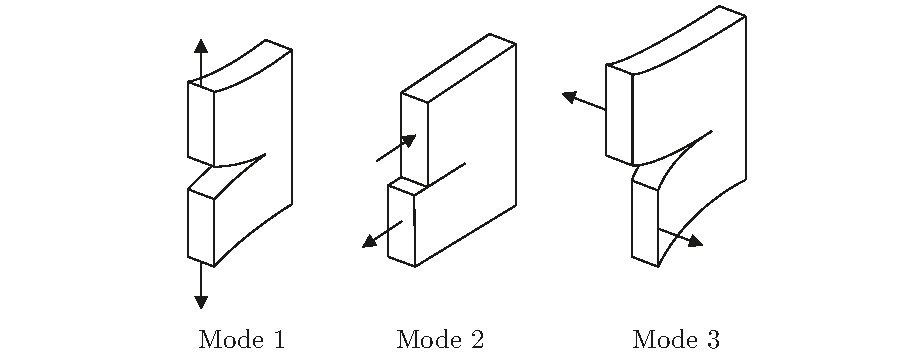
\includegraphics[width=10cm]{fig/fracture_modes.pdf}
        \caption{Fracture modes 1,2 and 3: opening crack, shearing crack and tearing crack}
        \label{FIGfracturemodes}
\end{figure}

In our brief tour through the approaches to the description of complex material behavior we only touch 
the problem by visualizing the source of the difficulties that are encountered when using material models 
formulated in the framework of plasticity and damage mechanics. 
These models are formulated in tensorial form and are based on the stress invariants described 
in in section~\ref{Sec:tensor_representation}. 

In the context of fracture mechanics, three fracture modes that we deal with can be distinguished: 
mode 1: opening crack, 
mode 2: shearing crack and mode 3: 
tearing crack (Fig~\ref{FIGfracturemodes}). 
A failure process containing a combination of fracture modes (mixed mode fracture) 
is characterized by interaction of 
fracture modes I and II, leading to the \textit{''mixed-mode''} fracture process. 
To motivate the detailed view to the problem, let us start with an experimental setup that has been designed
to render two symmetric cracks with combined tensile and shear loading. 
We will consider the analysis of the test performed on the double-notched specimen 
by Nooru-Mohamed~\cite{nooru_mixed_1992} and compare the behavior of the 
relatively widely ued concrete-damage-plasticity model implemented in Abaqus.
In parallel, we will introduce an alternative "non-tensorial" model using the
concept of microplane and explain its basic features.

We will then explore the model behavior using a verification test that studies the model behavior 
by defining loading paths within the principal stress space close to the yield condition. 
An extreme condition, occurs when moving through the stress space along a path parallel to the surface 
of the yield condition. Such loading path can be used to 
visualize pathological features of the models in general and to explain why a model is not able
to reflect the reality in some loading scenario.

To explain the better performance of the microplane-based modeling approach
we look at the fundametal concept of the microplane modeling approach at the end of the lecture.

\section{Double-edge notched test}

\mnote{Test setup} Nooru-Mohamed \cite{nooru_mixed_1992} tested square-shaped double-edge notched concrete 
specimens of $200\,\mathrm{mm} \times 200\,\mathrm{mm}$ with constant thickness 
of $t=50\,\mathrm{mm}$ subjected to different loading conditions (Fig.~\ref{FIGnoorumodamedtests}a). 
The bi-axial testing machine consists of two loading frames which can independently 
move in horizontal and vertical directions. 

\mnote{Loading scenario}
Test was performed in a sequence 
of transmitted loads $F_\mathrm{s}$ and $F$ using loading steel frames. At first, 
the test specimen was loaded in horizontal direction by force $F_\mathrm{s}$  
to a predefined level $F_\mathrm{s,max}$ at time $t_1$  (Fig.~\ref{FIGnoorumodamedtests}b). 
Then, the force $F_\mathrm{s}$  was kept constant and test specimen was loaded in vertical 
direction using displacement-controlled force $F$ up to the failure (Fig.~\ref{FIGnoorumodamedtests}c). 
Vertical displacement $\delta$ was measured using displacement gauges with the length 
of $t=65\,\mathrm{mm}$. Horizontal gauges were used to measure the displacement $\delta_\mathrm{s}$.

\begin{figure}
        \centering
        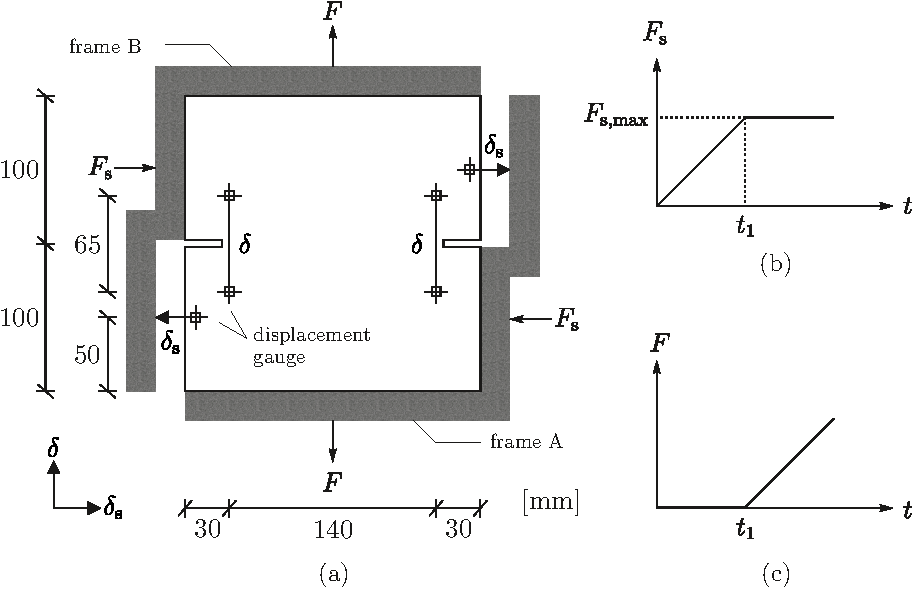
\includegraphics[width=12cm]{fig/nooru-mohamed-test-setup.pdf}
        \caption{(a) Test setup and dimensions of the Nooru-Mohamed tests; (b) loading history of horizontal force $F_\mathrm{s}$; (c) loading history of vertical force $F$}
        \label{FIGnoorumodamedtests}
\end{figure}

\mnote{Observed crack development}
Fig.~\ref{FIGnoorumodamedcracks} shows the test results for two different levels of the horizontal, shear-inducing force $F_\mathrm{s,max} = 5\,\mathrm{kN}$, and $F_\mathrm{s,max} = 10\,\mathrm{kN}$, respectively. Apparently, the described test setup and the applied loading history leads to a formation of rotating cracks. The low shear force $F_\mathrm{s,max} = 5\,\mathrm{kN}$ leads to almost horizontal evolution of cracks(Fig.~\ref{FIGnoorumodamedcracks}a), while the increased horizontal force of $F_\mathrm{s,max}= 10\,\mathrm{kN}$ induces curved cracks (Fig.~\ref{FIGnoorumodamedcracks}b). 

In the following paragraphs we compare the simulation results from two different material models, \textit{microplane damage model} and \textit{concrete damage plasticity model} from ABAQUS and discuss their ability to simulate the mixed-mode fracture. Finite element simulation of Nooru-Mohamed test is done using two-dimensional microplane damage model in combination with biquadratic elements of $2.5\,\mathrm{mm} \times 2.5\,\mathrm{mm}$.
%
\begin{figure}
        \centering
        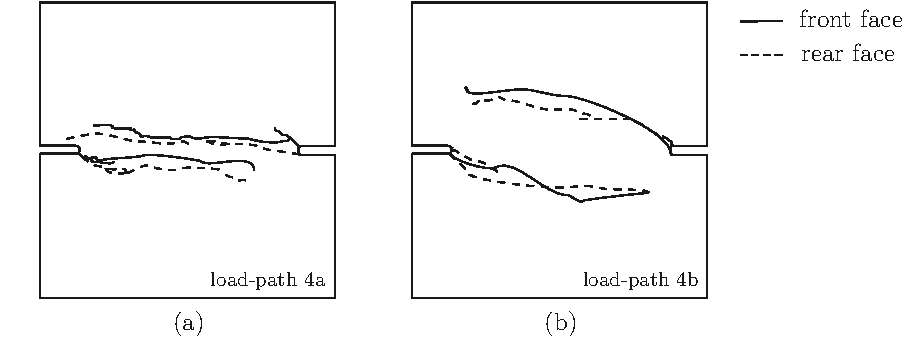
\includegraphics[scale=1]{fig/nooru-mohamed-cracks-test.pdf}
        \caption{(a) Crack pattern of Nooru-Mohamed test: (a) load path 4a; (b) load path 4b}
        \label{FIGnoorumodamedcracks}
\end{figure}

\subsection{Numerical simulation using concrete damage plasticity model}
\label{SEC:nooru-mohammed-CDP}

\paragraph{Brief characterization of the model}
This material model uses the concepts of isotropic damage in combination with plasticity. The stress-strain relation of the material in compression or tension is defined as
\begin{equation}
\boldsymbol{\sigma}=\left(1-\omega\right)\boldsymbol{D}^\mathrm{e}\left(\boldsymbol{\varepsilon} - \boldsymbol{\varepsilon}^\mathrm{pl} \right).
\label{EQCDPSigEps}
\end{equation}
In Eq.~\ref{EQCDPSigEps}, damage in the model is described using the scalar parameter $\omega \leq 1$ which is multiplied by the elastic stiffness tensor of the material $\boldsymbol{D}^\mathrm{e}$. In other words, the stiffness tensor of the damaged material $\boldsymbol{D}$ is obtained as $\boldsymbol{D} = \left(1-\omega\right)\boldsymbol{D}^\mathrm{e}$. All components of tensor $\boldsymbol{D}$ are reduced by the same factor $1-\omega$, regardlesly of the mode of loading (normal or shear).

\mnote{Material parameters}
Material model used for the simulation of Nooru-Mohamed tests are summarized in Table.~\ref{TABnoorumat}. For the modeling of the Nooru-Mohamed test using concrete damage plasticity model, the softening rule shown in Fig.~\ref{FIGnoorumohamedmdmcdpcal} was used. In this Figure, also a response of a single biquadratic element with reduced integration imposed to pure tension is shown for the $2.5\,\mathrm{mm} \times 2.5\,\mathrm{mm}$ mesh size. The obtained strain softening from \textit{concrete damage plasticity} model assures the same softening behavior and fracture energy as in microplane damage model under pure tension. Further parameters required for the \textit{concrete damage plasticity} model are dilation angle $\theta = 35^\circ$, eccentricity $\epsilon = 0.1$, $\frac{\sigma_{b0}}{\sigma_{c0}}=1.16$ and $K_c=\frac{2}{3}$.
%
\begin{table}\centering
\caption{Material parameter for simulation of Nooru-Mohamed tests}
%\renewcommand{\arraystretch}{1.3}% Wider
\begin{tabular}{l ccc}
        \textbf{Description} & \textbf{Symbol} & \textbf{Value} & \textbf{Unit}\\
  \hline
	elasticity modulus & $E$ & $29000$ & $\mathrm{N/mm^2}$ \\
  tensile strength & $f_\mathrm{t}$ & $3.0$ & $\mathrm{N/mm^2}$ \\
  fracture energy & $G_\mathrm{f}$ & $0.11$ & $\mathrm{N/mm}$ \\
\end{tabular}
\label{TABnoorumat}
\end{table}
%
\begin{figure}
\centering
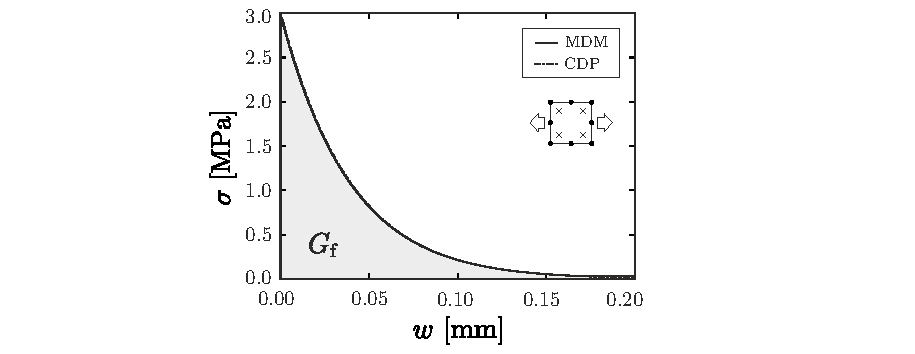
\includegraphics[scale=1]{fig/nooru-mohamed-mdm-cdp-cal.pdf}
\caption{Tensile response of Microplane damage model (MDM) and Concrete damage plasticity (CDP) calibrated for the simulation of Nooru-Mohamed tests}
\label{FIGnoorumohamedmdmcdpcal}
\end{figure}

\mnote{Simulation results}
Evolution of damage obtained by the simulation using \textit{concrete damage plasticity} model is compared to the crack pattern of the test for load paths 4a and 4b. Considering the load path 4a, the results are sufficiently good compared to the test. The good conformity with the test results justifies the capability of the \textit{concrete damage plasticity} model in realization of fracture mode I with minor shear force included. Now considering the load path 4b, once the shear force $F_\mathrm{s}$ becomes proportionally larger than load path 4a, the model is unable to realize the mixed-mode fracture. The model is obviously unable to represent the inclined and rotating for of the crack pattern.
%
\begin{figure}
\centering
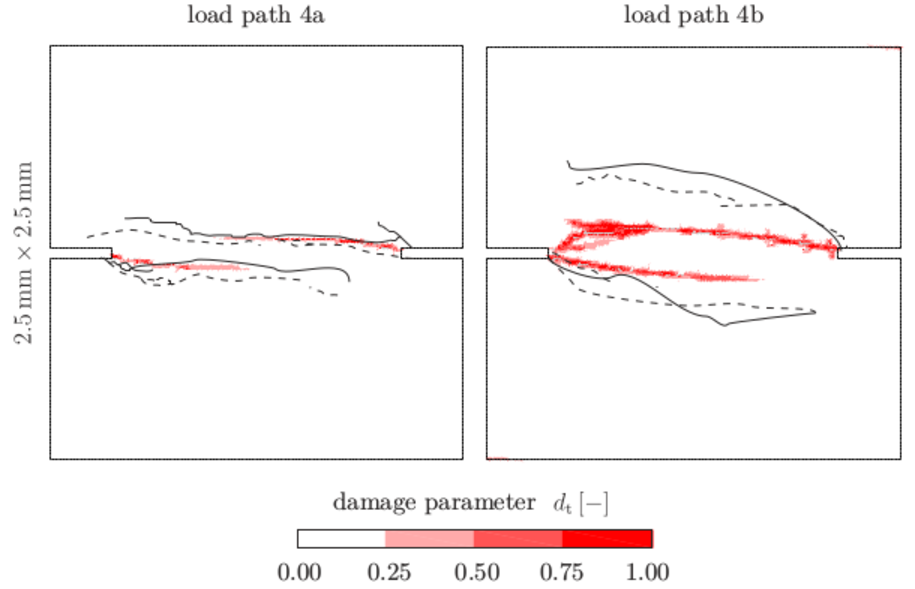
\includegraphics[width=12cm]{fig/nooru-mohamed-cracks-cdp.pdf}
\caption{Comparison of the crack pattern in Nooru-Mohamed test (load paths 4a and 4b) with damage evolution from the model with biquadratic elements with $2.5\,\mathrm{mm} \times 2.5\,\mathrm{mm}$ mesh size and reduced integration schemes using \textit{concrete damage plasticity} model}
\label{FIGnoorumodamedcrackcdp}
\end{figure}

The load displacement curves of $F-\delta$ are shown in Fig.~\ref{FIGnoorumodamedfdeltacdp}.
\begin{figure}
\centering
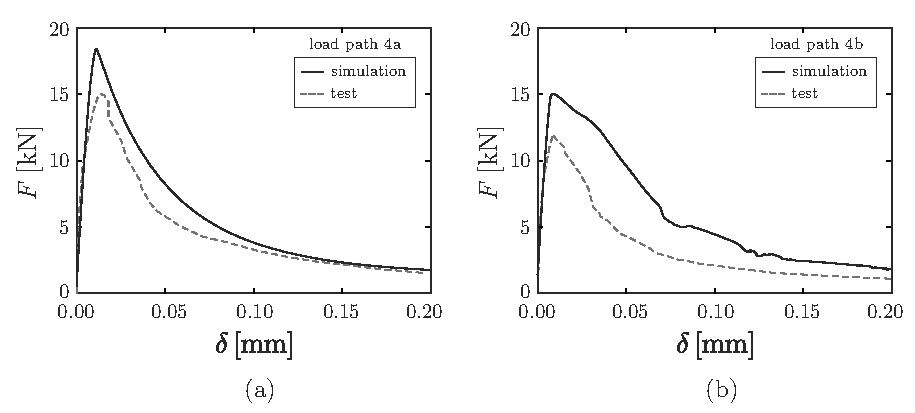
\includegraphics[scale=1]{fig/nooru-mohamed-f-delta-cdp.pdf}
\caption{Load-displacment curves of the Nooru-Mohamed test from test and finite element simulation using \textit{concrete damage plasticity} model (a) load path 4a; (b) load path 4b}
\label{FIGnoorumodamedfdeltacdp}
\end{figure}

\subsection{Numerical simulation using 
\textit{microplane damage model}}

\mnote{Brief characterization of the model}
The principle idea behind the microplane damage model is to formulate the damage not-within the stress invariants but to resolve the stress state in a material point into indvidual directions. The concept is indicated in Fig.~\ref{FIGMicroplane-disc}.
\begin{figure}
\centering
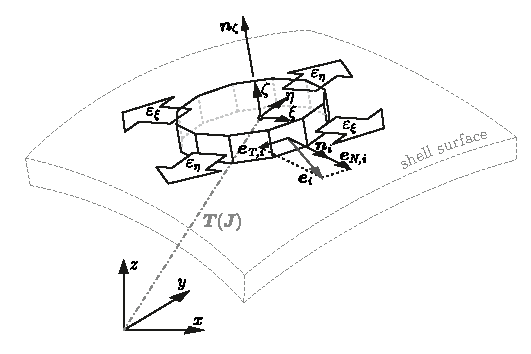
\includegraphics[scale=1]{fig/TRC_disc.pdf}
\caption{Decomposition of strain components in a material point in 2D stress state.}
\label{FIGMicroplane-disc}
\end{figure}
\begin{figure}
\centering
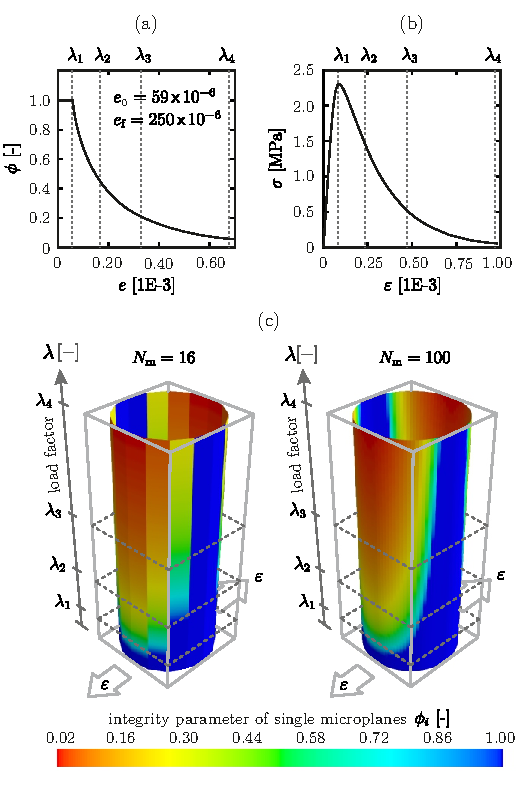
\includegraphics[width=10cm]{fig/Damage_plot_cylinder.pdf}
\caption{Example of damage evolution in a material point loaded in uniaxial tension.}
\label{FIGMDM_damage_cylinder}
\end{figure}

Then, the damage function is not related to all strain components equally, but is related to a direction on a circle or sphere.
Therefore, an anisotropic damage evolution can be described and in this way also an emerging, oriented crack.
Fig.~\ref{FIGMDM_damage_cylinder} shows an example of a single material point loaded in tension. The loading factor $\lambda$ is plotted along the vertical axis of the cylinder. Thus, the changing indicate the evolution of damage with the increasing level of loading. The directions oriented in perpendicular direction with respect to the loading direction are almost undamaged. In this way, the material model can describe an oriented crack.
This model belongs to the category of anisotropic damage models but possesses a clear geometrical interpretation of the material point state.

It is useful to set the model into the context of the models formulated in tensorial form with an explicitly defined failure surface within the principal stress space. The failure envelope can be calculated by repeated simulations with different ratios of the strains $\varepsilon_{xx}$ and $\varepsilon_{yy}$.
\begin{figure}
\centering
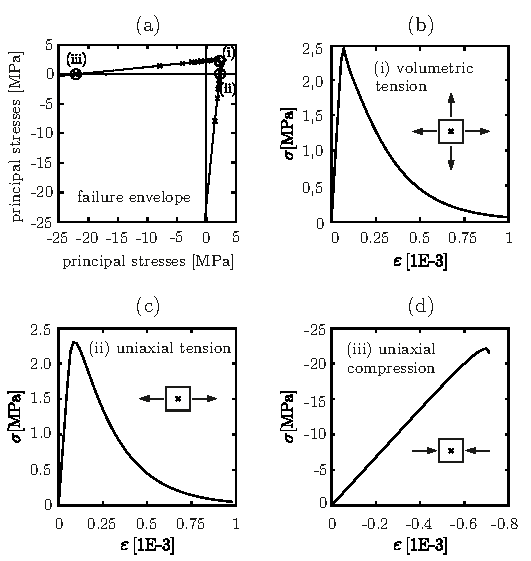
\includegraphics[width=12cm]{fig/Damage_envelope.pdf}
\caption{Damage envelope calculated for the microplane-damage model.}
\label{FIGMDM_damage_envelope}
\end{figure}
Fig.~\ref{FIGMDM_damage_envelope}a shows the cut through the plane stress plane. The other three stress-strain diagrams shown in Figs.~\ref{FIGMDM_damage_envelope} show the response for biaxial tension (a), uniaxial tension (b), and uniaxial compression (c). Note that, this version of the model does not define an envelop for biaxial compression. 

\mnote{Material parameters}
The material parameters needed for the present version of the microplane model were set equivalent to the parameters used for the concrete damage-plasticity model given in Table.~\ref{TABnoorumat}. The input for the microplane model is represented by the damage function defined at the microplane level. In order to achieve equivalence, of calculation, we need to ensure the same fracture energy dissipation for both models. 


\mnote{Simulation results}
Fig.~\ref{FIGnoorumodamedcrackmdm} shows the evolution of damage in the finite element simulation using biquadratic elements with comparison to the crack pattern from the test for load path 4a and 4b. Results from Fig.~\ref{FIGnoorumodamedcrackmdm} give clearer localization zone with crack branches going across the mesh diagonals compared to the results obtained from Fig.~\ref{FIGnoorumodamedcrackcdp}.
The load displacement curves of $F-\delta$ are shown in Fig.~\ref{FIGnoorumodamedfdeltamdm}.
Apparently, a better match between the predicted and calculated crack geometries has been achieved as compared to the concrete damage plasticity model described in Sec.~\ref{SEC:nooru-mohammed-CDP}.

\begin{figure}
\centering
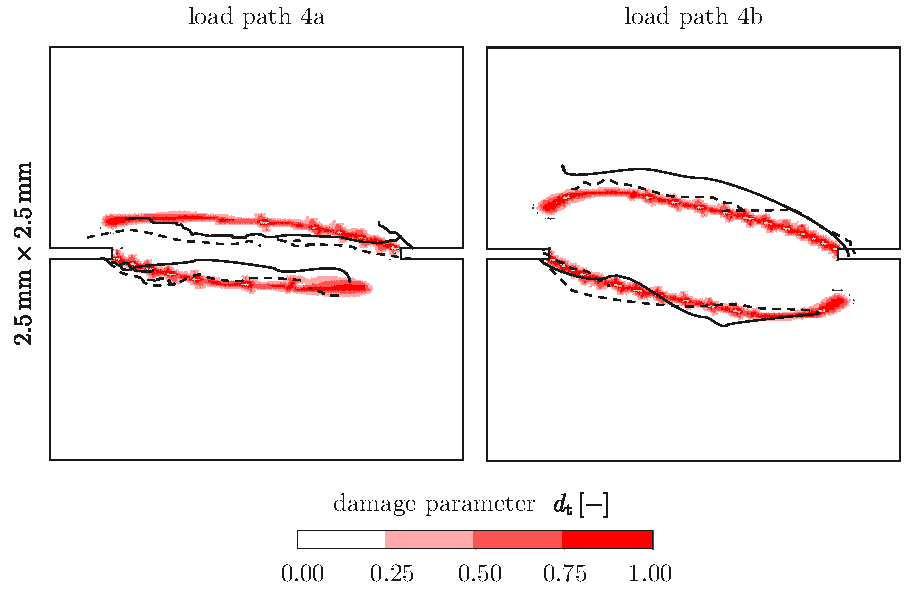
\includegraphics[width=15cm]{fig/nooru-mohamed-cracks-mdm.pdf}
\caption{Load-displacment curves of the Nooru-Mohamed test from test and finite element simulation using \textit{microplane damage model} (a) load path 4a; (b) load path 4b}
\label{FIGnoorumodamedcrackmdm}
\end{figure}

\begin{figure}
\centering
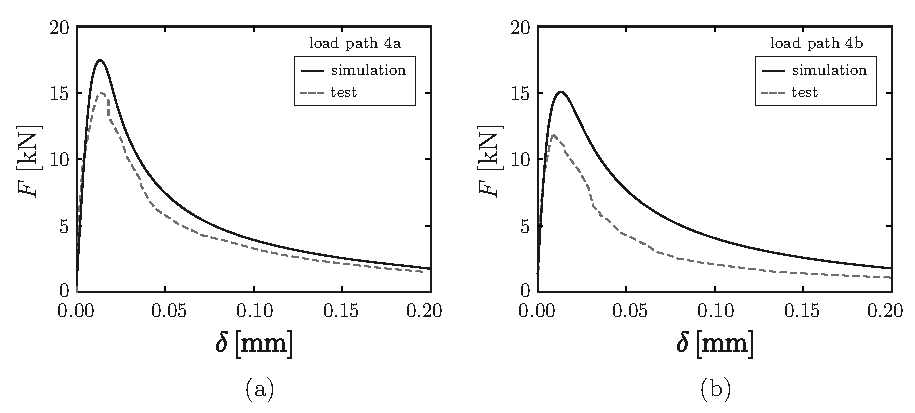
\includegraphics[scale=0.9]{fig/nooru-mohamed-f-delta-mdm.pdf}
\caption{Load-displacment curves of the Nooru-Mohamed test from test and finite element simulation using \textit{microplane damage model} (a) load path 4a; (b) load path 4b}
\label{FIGnoorumodamedfdeltamdm}
\end{figure}

In order to shed some light onto the large number of model formulations
and to provide better understanding about the validity of individual models
provided in commercial codes we discuss the tests focusing on the combined
tensile and shear loading. 
On the one hand elementary verification tests, that can discover pathological behavior of models are available. 
On the other hand, validation tests provide the information on to what extent can the model predict the real behavior of a structure. 
 
\section{Elementary tests of material models for concrete cracking}

The present example with mixed-mode crack development indicates the difficulty 
to describe an inelastic behavior leading to crack localization for highly non-proportional loading paths with rotating principal stress axes. 
The  classical  tensorial  models  of  plasticity  type fail to correctly predict  the behavior for such  loading scenarios.

To illuminate the effect and to provide a general test for quality assessment of the developed models, elementary numerical tests have been proposed in the past. An combining tensile loading with subsequent shear has been proposed Willam test \cite{willam1989fundamental} combining tensile loading with subsequent shear. This test illuminates the core of the problem for tensorial material models formulated in the framework of plasticity and softening. Another example is a vertex test combining a compressive loading with a subsequent loading traveling parallel to the yield surface. In both these cases,   principal strain  or  stress  axes  rotate  against  the  material \cite{caner2002vertex}.

Let us examine the behavior of the two models considered in this lecture for combined tension and shear.

\subsection{Willam test}

The
loading history of Willam’s test is characterized by uniform tensile loading followed by shear
loading leading to a rotation of principal strains. Basically, Willam’s test is passed when 
\begin{itemize}
\item the
maximum principal stress is always lower than or equal to the uniaxial tensile strength ftu of
concrete and 
\item all stress components tend to zero.
\end{itemize}

\begin{figure}
\centering
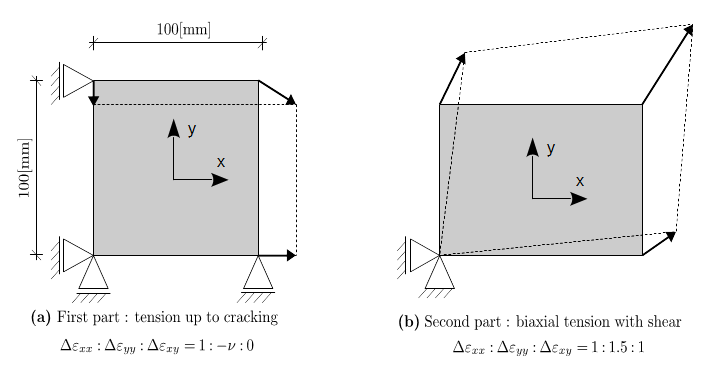
\includegraphics[width=12cm]{fig/Willam-test-illustration.png}
\caption{Willam test illustration}
\label{FIGWillamTestIllustration}
\end{figure}

\begin{figure} 
    \centering
    \begin{subfigure}[b]{0.4\textwidth}
        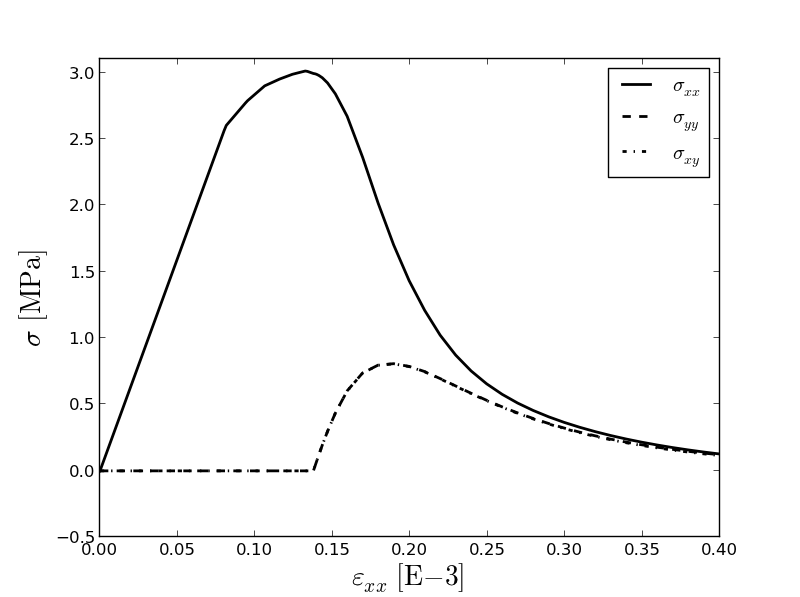
\includegraphics[width=7cm]{fig/WillamTest-Sig-Eps11-CDP.png}
        \caption{Concrete-damage plasticity, Abaqus}
        \label{FIGWillamTestSigEps}
    \end{subfigure}
    \begin{subfigure}[b]{0.4\textwidth}
        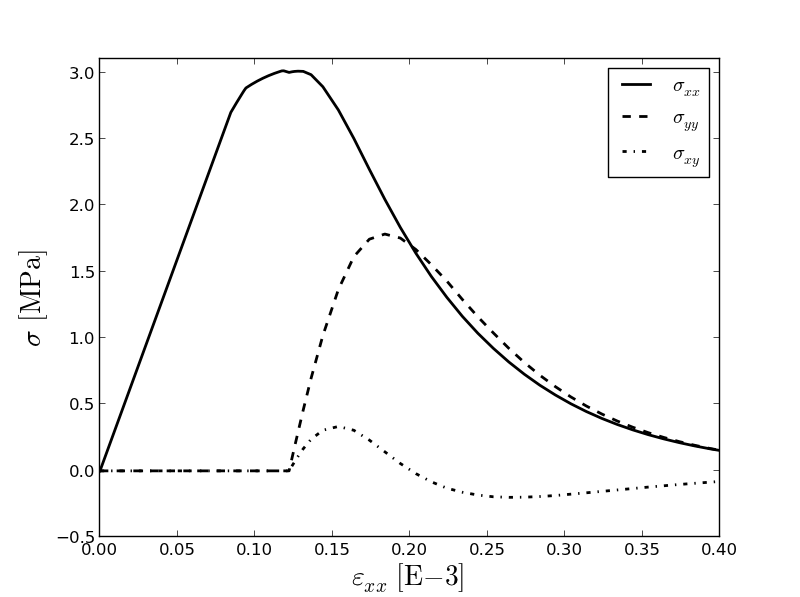
\includegraphics[width=7cm]{fig/WillamTest-Sig-Eps11-MDM.png}
        \caption{Microplane damage model}
        \label{FIGWillamTestSigEps}
    \end{subfigure}
    \caption{Willam-test, $\sigma_{xx}, \sigma_{yy}, \sigma_{xy}$ versus $\varepsilon_{xx}$}
\end{figure}

\begin{figure} 
    \centering
    \begin{subfigure}[b]{0.4\textwidth}
        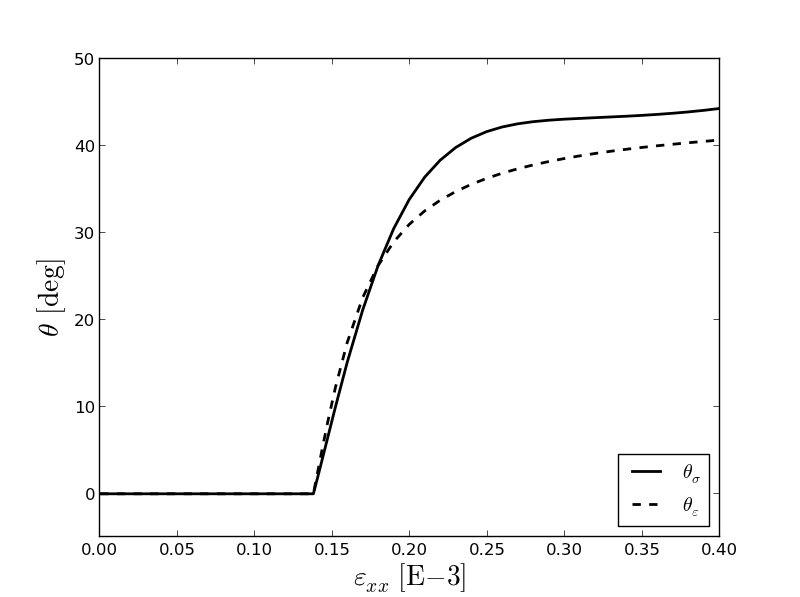
\includegraphics[width=7cm]{fig/WillamTest-Theta-Eps11-CDP.png}
        \caption{Concrete-damage plasticity, Abaqus}
        \label{FIGWillamTestSigEps}
    \end{subfigure}
    \begin{subfigure}[b]{0.4\textwidth}
        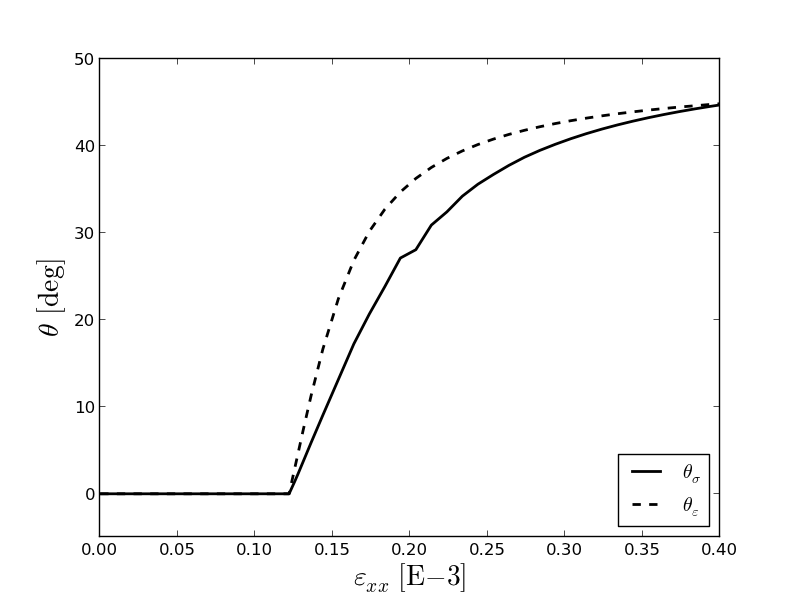
\includegraphics[width=7cm]{fig/WillamTest-Theta-Eps11-MDM.png}
        \caption{Microplane damage model}
        \label{FIGWillamTestSigEps}
    \end{subfigure}
    \caption{Willam-test, evolution of directions of principal stress $\sigma_{11}$ and 
    strains $\varepsilon_{11}$}
\end{figure}

\begin{figure} 
    \centering
    \begin{subfigure}[b]{0.4\textwidth}
        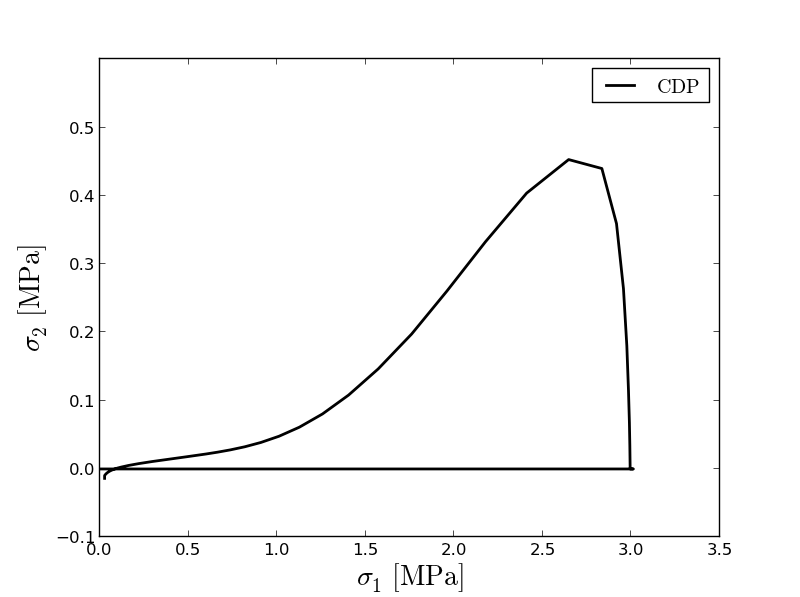
\includegraphics[width=7cm]{fig/WillamTest-Sig1-Sig2-CDP.png}
        \caption{Concrete-damage plasticity, Abaqus}
        \label{FIGWillamTestThetaCDP}
    \end{subfigure}
    \begin{subfigure}[b]{0.4\textwidth}
        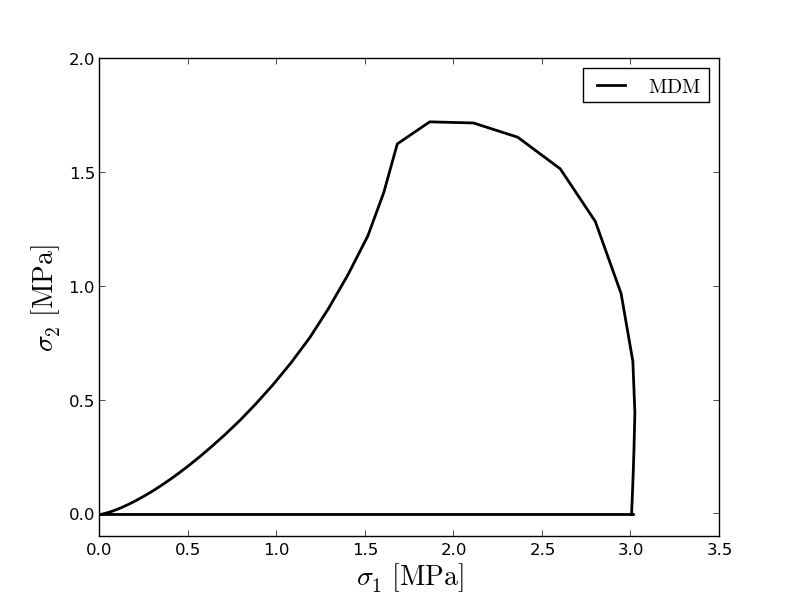
\includegraphics[width=7cm]{fig/WillamTest-Sig1-Sig2-MDM.png}
        \caption{Microplane damage model}
        \label{FIGWillamTestThetaMDM}
    \end{subfigure}
    \caption{Willam-test, evolution of principal stresses}
\end{figure}

\end{document}